\chapter{FDI}
\label{chap:FDI}

\section{FDI trends}

Intro about studies of FDI in political science

Write about the economic literature on determinants of FDI

The political economy literature on the political determinants of FDI (and that
paper who shows that the political factors are not that important)

The studies on the preference of countries about FDI (Pandya, Pinto, and the
Harvard pub pol paper)


\section{Introduction}
\label{sec:introduction}

The political science literature on Foreign Direct Investment (FDI) has focused
largely on how politics shapes the flow of FDI across countries. The central
insight of this literature is that multinational corporations (MNCs) face an
``obsolescing bargain'' against the host government. Once the MNC has sunk its
investment, it is vulnerable to the host government's changing regulations,
backtracking on deals, or even expropriating its properties \citep{Li2009a,
Sawant2010}. Certain institutional and political characteristics, such as
numerous veto players, executive constraint, or strong property rights, allow
the host government to make a credible commitment and thus ameliorate the
severity of the ``obsolescing bargain'' problem \citep{Busse2007, Jensen2014,
Li2003}. According to the literature, MNCs should invest more in countries with
these characteristics.

This dominant approach in the literature has three long-standing issues that my
paper will address. First, the majority of the literature relies on FDI stock
and flow data as the outcome of interest even though they are often not an
appropriate measure for the scale of MNCs' activities \citep{Kerner2014}. While
it would be ideal to use firm-level data instead, both the lack of
cross-national firm-level data and a suitable statistical model have posed a
challenge.

Second, while there has been much focus on MNCs choosing host countries, the
literature has largely neglected the other side of the investment decision: what
are countries' preferences regarding MNCs? Consider the established finding that
democracies receive more FDI. Without controlling for countries' preferences, it
is difficult to interpret this fact as democracies actively pursuing MNCs or as
MNCs finding democracies attractive. Not only are countries' preferences central
to the modeling of investment decision, arguably it is also more steeped with
politics and deserves more attention. \citet{Pinto2013} and \citet{Pandya2016}
are two pioneering works in this area of research, proposing partisan politics
and regime types as factors shaping countries' preferences for FDI. However,
while their theories are ground-breaking, the empirical estimation of countries'
preferences remains difficult.

Third, in addition to empirical issues raised above, I propose that we need to
theorize about countries' preferences for FDI quality. While the political
science literature has largely focused on the quantity of FDI, national policies
and discourses pay much attention to the quality of FDI, using various
incentives and restrictions to target certain types of FDI. Indeed, MNCs come
with varying capital, demand for labor, and technology, all of which have
different effects on the host country's economy. For example, policy makers and
scholars have highlighted high-tech MNCs as a source of technological transfer
for developing host countries, allowing them to upgrade their technical capacity
and improve their productivity \citep{Findlay1978, Nunnenkamp2004}. While such
high-quality FDI has been enthusiastically endorsed by the development
community, I argue that only governments with a long time horizon want to
attract high-tech FDI because technological transfer takes time to pay off.

In sum, the current literature would benefit from an analysis that is capable of
using firm-level data to estimate both firms' and countries' preferences for
each other's characteristics. To accomplish this goal, I adapt the two-sided
matching model originally designed for the labor market and the marriage market.
In this model, both firms and countries evaluate their available options and
choose the best according to their utility functions. As in many social science
contexts, we only observe the final firm-country matches and not the full set of
available options (also known as the opportunity set). I solve this problem by
using the Metropolis Hastings algorithm, a Markov chain Monte Carlo (MCMC)
approach that repeatedly samples new opportunity sets and rejects them at an
appropriate rate to approximate their true distribution. Since the two-sided
matching model is derived explicitly from actors' utility functions, their
parameters also enjoy a straightforward interpretation in the utility space
instead of some aggregate outcomes.

The paper proceeds as follows. Section \ref{sec:literature_issues} discusses the
three long-standing issues with the literature and how they can be improved.
Section \ref{sec:model} lays out the utility structure in the two-sided matching
model and describes the matching process. Section \ref{sec:application} shows an
application of the model on a census of Japanese firms overseas. Section
presents the result. Section \ref{sec:conclusion} concludes.

\section{Three Issues in the Literature of FDI's Political Determinants}
\label{sec:literature_issues}

Using flow: \citep{Jensen2005}: democracy and federalism -> more FDI flow (panel
data), \citep{Jensen2008}: tax rate does NOT matter for FDI flow (OECD),
\citep{Busse2007}

(I use manufacturing FDI, so most capital in manufacturing is fixed) (because of
the the ``obsolescing bargaining'' argument. )


\subsection{Measuring MNCs' Activities}

As \citet{Kerner2004} argues, the political economy literature on FDI is a bit
of a misnomer. Political scientists are rarely interested in FDI \textit{per
se}---rather, they are interested in the activities of MNCs, which in turn,
affect other important issues such as nation-state autonomy \citep{Mosley2005},
economic development \citep{Moran1998}, labor standards \citep{Mosley2007}, and
environmental policies \citep{Prakash2007}. However, while the theories involve
MNCs as the central actor in the causal mechanism, the empirics often use FDI
flow as the independent variable of interest. These two concepts---the level of
MNCs' affiliate activities in a country and FDI inflow into a country---are not
the same.

Consider the definition of FDI from UNCTAD, the main producer of FDI data widely
used by researchers:

\begin{quote} FDI has three components: equity capital, reinvested earnings and
intra-company loans.
\begin{itemize}
\item Equity capital, i.e. the foreign investor’s purchase of shares of an
enterprise [in the host country].
\item Reinvested earnings, i.e. the foreign investor’s share \ldots of earnings
not distributed as dividends by affiliates, or earnings not remitted to the
foreign investor.
  \item Intra-company loans between direct investors and affiliate enterprises.
\end{itemize} \citep[245]{UNCTAD2007}
\end{quote}

In essence, FDI data captures the amount of capital that crosses border. It is a
poor proxy for the scale of MNCs' activities in the host countries because it
overlooks important components of MNCs' activities while including components
that are only relevant for balance of payment statistics
\citep{Beugelsdijk2010}.

Consider the argument that FDI is the driver for the diffusion of labor
standards across countries. \citet{Mosley2007} theorizes that FDI can have this
effect through three channels. First, MNCs may pressure the host governments for
better rule of law and social programs. For MNCs to be able to effectively
pressure the host governments, they must prove themselves valuable to the
government by providing jobs or tax revenues. Both of these factors are only
tenuously related to the amount of foreign capital inside the host country.
Indeed, a MNC can employ thousands of employees, pay millions in tax, but show
up as a net 0 on FDI flow data because the profit is repatriated to the foreign
investor or through intra-company loans.\footnote{The issue of intra-company
loans is particularly fraught with issues because companies very frequently use
intra-company loans to get out of paying tax in a country. These loans will be
recorded on the book as a massive outflow, even though the MNC still has a large
presence on the ground.} The size of the MNCs' operation is further understated
because FDI statistics does not take into account capital raised locally. It
also does not take into account the productivity of MNCs, which acts as an
important multiplier when translating the amount of capital to the amount of
output.

Second, scholars argue that MNCs may bring along best practices for workers'
rights and spread it to local firms. If this channel operates via competition as
MNCs provide better working condition forcing local firms to compete, then MNCs
must employ a lot of labor for this effect to be noticeable. If this channel
operates via demonstration, then it must form a lot of linkages with local
firms, as suppliers and buyers, for the diffusion of norms to happen. Both the
size of the labor force and the type of linkages with the local economy are not
captured by FDI flow statistics.

Third, scholars argue MNCs may care more about labor quality than its cost, and
thus may invest in higher wages, better benefits, or more training. Once again,
for this effect to be noticeable, the size of the MNCs' labor force matters, its
industry, and its investment in productivity, matters a lot more than how much
capital it brings in and out of the country. In addition, non-equity
transactions between the foreign parent company and the local subsidiary are not
counted in FDI flow statistics, such as transfer of knowledge, technology, and
management practices, thus excluding a component that is arguably much more
important to labor quality than the amount of capital.\footnote{These issues are
not isolated to studies of FDI and labor standards, but are common to the whole
IPE literature of the effect of FDI on policy convergence, such as environmental
policies \citep{Prakash2007}.}

This mismatch may also be a reason behind the still unsettled debate on the
effect of FDI on poverty reduction. Scholars have theorized that FDI can lead to
economic development and through three channels. First, MNCs can simply provide
cheaper and better goods by being more productive. Second, MNCs may improve the
productivity of local economy through technology transfer. Finally, MNCs can
bring tax revenue to the host government, which can then spend on the poor via
investment into social programs. Once again, these causal mechanisms only work
depending the scale and the type of MNCs activities in the host country, not on
the amount of equity capital that crosses the border. For example, productivity
spillover is highly conditional on how thick the linkages between the MNCs and
the local suppliers are as well as how technologically advanced the MNCs'
activities are on the ground. The effect of FDI via tax revenue is particularly
fraught with issues, as MNCs frequently engage in transfer pricing to get out of
paying tax, especially via intra-company transactions of goods and services,
such as charging for internal IP, whose price can be set arbitrarily by the firm
\citep{Malesky2015c}, which are not recorded in FDI flow statistics, \footnote{A
similar argument is about the relationship of FDI on economic development,
especially on the technology spillover and tax revenue.}

What about studies that use FDI as the dependent variable, and are thus perhaps
interested in flow of capital in and of itself?\footnote{Arguably, political
scientists are not interested in the flow of capital in and of itself, but also
because of its implications for development, state autonomy, and other effects
on policy. The discussion above has shown how problematic it is to study these
effect of FDI using FDI flow data.} The vast majority of theories on the
political determinants of FDI flow relies on the ``obsolescing bargain'' model.
Originally developed by \citet{Vernon1971}, the model is so named because the
bargaining dynamics between the MNC and the host government changes over time,
initially favoring the MNC and gradually tips towards the host government as the
MNC commits more fixed capital on the ground. Indeed, knowing that it is costly
for the MNC to uproot its increasingly large and immobile operation, the host
government can unilaterally alter the original bargain, most egregiously by
expropriating the MNC's asset and profit, but more often via ``creeping
expropriation,'' e.g. increased tax or tougher regulation \citep{Li2009a}.
Political economists argue that MNCs are acutely aware of the ``obsolescing
bargain,'' and thus prefer to invest in countries whose governments can make a
credible commitment that they will not alter the original bargain. This means
MNCs prefer countries with democratic accountability \citep{Jensen2003}, a
federal system \citep{Jensen2005}, membership in international trade agreements
\citep{Buthe2008}, less political risk \citep{Beazer2011, Graham2010}, or more
veto points \citep{Choi2008}.\footnote{The fact that FDI is understood as
illiquid capital subject to the obsolescing bargain is the central theoretical
difference between FDI and footloose equity capital \citep{Ahlquist2006,
David2008}}.

The linchpin of this argument is the assumption that FDI capital is illiquid and
cannot be quickly removed from the host country at will. This assumption is not
fully warranted. According to the US Bureau of Economic Analysis (BEA)'s 2004
survey, 43\% of US MNCs' balance sheet comprises of liquid assets that can be
liquidated within one year under normal operating situations. Among the 57\% of
the balance sheet that are illiquid, 24\% are ``other non-current assets,''
which include non-tangible assets like brand names, trademarks, and
patents---some of which are not expected to be liquidated but can be removed
from the host countries. Only another 24\% of the balance sheet is made up of
physical capital, i.e. Plant, Property, and Equipment (PPE), which cannot be
easily moved and match most closely to what we have in mind as the ``illiquid
capital'' in the obsolescing bargain model \citep[113]{Kerner2014a}.

Besides the conceptual mismatch between FDI flow and MNCs' activities, from a
statistical standpoint, this measurement error may also be a contributing factor
to the still unsettled debate on the effect of FDI. Even when the measurement
error is random, it will inflates the standard error of our estimate when FDI is
the dependent variable, and bias our estimate towards 0 when FDI is the
independent variable. These effects may explain \citet{Jensen2012}'s surprising
finding that lower corporate tax rate does not lead to more FDI flow, or the
mixed empirical evidence for the relationship between FDI and development
\citep[108]{Mold2004}.

Even more worryingly, the measurement error is unlikely to be random. For
example, the amount of locally raised capital, something we care about but FDI
statistics does not capture, is likely to correlate with how developed the local
capital market or the fluctuation in the exchange rate. On the other hand,
repatriated earnings, something that does not necessarily indicate reduced MNCs'
activities but is recorded as an outflow in FDI statistics, is likely to
correlate with the tax rate of not only the host country but also the tax rate
of tax havens that the MNC may have an affiliate in.\footnote{See
\citet{Gallop2017} for a recent and more comprehensive discussion of measurement
error in political science research.} \footnote{FDI stock calculated at market
value fluctuates based on market price, unrelated to firms' behavior. FDI stock
calculated at historical value, which records asset value at the time it was
acquired, is more stable and appropriate to measure the scale of MNCs'
activities. Unfortunately, due to onerous data requirements, most countries
measures FDI stock by simply adding up FDI flow across years. See
\citet[809]{Kerner2014} for a more in-depth discussion of FDI stock and flow
data.}

To deal with the measurement error problem, scholars have tried to use
measurements that are closer to the theory than FDI flow. Given that political
scientists are interested in MNCs' activities, recent work emphasizes using
MNCs' operational data directly. These firm-level data allow researchers to
measure directly the quantities of interest. For example, re-visiting
\citet{Li2009a}'s hypothesis that democracies are more attractive to MNCs,
\citet{Kerner2014} uses data on US MNCs' fixed capital expenditures to more
precisely test the relationship between democratic institutions and
\textit{illiquid} capital, not just FDI in general. The author finds that there
is no relationship between democratic institutions and FDI flow and stock, but
there is a positive relationship between democracy and MNCs' fixed capital
expenditures, confirming the theoretical argument \footnote{Another alternative
is to use other variable, for example when \citet{Jensen2008} re-examines
whether MNCs favor democratic regimes because they pose less political risk, the
author avoids using FDI flow and use price data of political risk insurance
agencies instead. In other areas of IPE, scholars are also paying more attention
to using the data that maps more closely to the theoretical argument, e.g.
\citep{Karcher2013}.}

In another example, \citet{Arel-Bundock2017} uses ORBIS data to study the location decision of
firms. However it only does one sided (i.e. only looking at the characteristics
of the host countries to predict incidence of investment). This is a bit of a
missed opportunities because using his Random Forest / non-parametric approach,
it would have been possible to incorporate characteristics from firms. Then the
random forest would be able to take into account the interactions between the
firms' characteristics and country characteristics (in the form of sequential
tree split). Even then, since random forests do not produce interpretable
coefficients, this black-box approach does not allow us to understand the
preference of actors, how these preference are correlated with other
characteristics, and how they may evolve over time. The only claim he can make
is whether some factors add predictive power over other factors.

In sum, while the need to use better data is clear, and while firm-level data has become more abundant in recent
years,\footnote{Examples of firm-level data include the US Bureau of Economic
Analysis (BEA)'s survey of all US firms abroad, Tokyo Keizai's Overseas Japanese
companies database (\textit{Kaigai Sinshutsu Kigyou Souran}), World Bank's
Enterprise Survey, and Orbis database of companies worldwide.} political
scientists have not developed a model to estimate this data appropriately. Given the data structure of a
set of firms interacting with a set of countries, one may consider a
dyadic-based analysis, frequently used in the International Relations
literature. In such analysis, the unit of observation is a firm-country dyad,
and the model used is typically OLS regression. Each dyad is assumed to be
independent of each other, and any bias caused by interdependency is fixed via
post-estimation procedures, such as clustered standard errors \citep{Dorff2013}.

Unfortunately, this dyadic approach is inappropriate to analyze MNCs' investment
location. Once a firm chooses to invest in a country, it is by definition not
investing in another. Therefore, the values of firm-country dyads
deterministically constrain one another and cannot be modeled as independent
draws from a common distribution.

The two sided matching model solves this problem by considering one firm-country
match as the unit of observation. The intuition is as follows. If we observe
that a firm is welcome to invest in countries $j_1, j_2, \dots, j_n$ but ends up
investing in country $j^*$, it must mean country $j^*$ offers the highest
utility to firms. Continuing the previous example, if country $j^*$ has more
veto players than average, we can infer that MNCs indeed prefer countries with
more veto players.

\subsection{Estimating Countries' Demand for FDI}

Recognizing that our model of investment location has not taken into account
countries' demand for FDI, \citet{Pinto2013} and \citet{Pandya2016} recently
broke ground in this area. Similar to the rich IPE literature in trade and
exchange rate, these studies argue that countries' demand for FDI varies
according to FDI's distributive effect on their domestic constituencies
\citep{Broz2001, Milner2005a}. In this theoretical framework, labor supports FDI
because foreign firms bring capital that increases the demand for labor and
raises productivity, both of which lead to higher wage. On the other hand,
domestic firms oppose FDI because foreign firms compete for local labor, inputs,
and markets. Both \citet{Pinto2013} and \citet{Pandya2016} formulate their
theories as a variant of this labor-vs-business tension, which surfaces in the
former work as left-vs-right governments, and in the latter as
democratic-vs-authoritarian regimes.

While these pioneering works have enriched our understanding of the relationship
between politics and FDI, their empirical approaches do not satisfactorily
measure countries' demand for FDI, leaving their theoretical arguments untested.

Consider \citet{Pinto2013}'s approach, which controls for economic and
institutional factors that affect FDI flow into a country. The author then
claims that the country's openness towards FDI is what's left in the
residual.\footnote{Specifically, the estimation of FDI openness involves two
steps. First, the author runs a gravity model explaining bilateral FDI flows,
estimating the intercept as the host country-year fixed effect. Second, this
fixed effect is then regressed on several economic and endowment factors of that
country-year (i.e. GDP, GDP per capita, average school years, arable land). The
residual in the second stage is considered the country's ``FDI openness'' in
that year.} For this approach to be valid, every economic, institutional, and
endowment factors that affect FDI flow have to be controlled for, leaving only
the country's demand in the error term. This claim is much stronger than the
regular assumption of exogenous and normally distributed error, which is valid
as long as the omitted factors are uncorrelated with the independent variable of
interest. Framed substantively, since the residual is likely to contain more
than just the country's demand for FDI, if we observe an abnormally high level
of FDI, we do not know whether it is because the country welcomes FDI or because
MNCs find something attractive in the country.\footnote{In addition, the data
requirement of bilateral FDI flows, ideally disaggregated by sectors, is very
demanding. Therefore, this approach is limited to OECD countries only
\citep{Pinto2008}. During the period the authors study, 1980-2000, OECD
countries accounted for 95\% of global FDI outflow and 90\% of inflow. However,
since then the role of the developed world in global FDI has declined sharply,
reduced to 60.8\% of outflow and 40.6\% of inflow in 2014 \citep{UNCTAD2015}.}

In contrast to \citet{Pinto2013}'s statistical approach, \citet{Pandya2014,
Pandya2016} substantively measures countries' demand for FDI, using the annual
US Investment Climate Reports to code the number of industries that have foreign
ownership restrictions or face investment screening. The advantages of this
measurement are its ease of interpretation and its availability for many
countries. However, two problems remain. First, adding up the raw count of
restricted industries is not appropriate because industries are not all the
same. For example, given the reach of the banking sector into all corners of the
economy, a country's opening up its financial industry indicates much more
FDI-friendliness than, say, allowing foreign furniture makers to set up shops.
Since the theoretical argument is driven by FDI's distributive effect, it is
suspect to ignore the varying impact of FDI across sectoral constituencies.

Second, according to the coding rules, an industry is coded as free if there is
no mention of restriction. If an industry receives little FDI, it may not be
worth mentioning as being restrictive and yet still coded as open. Therefore,
``zero restriction'' in the dataset can either mean that a country is very
closed or very open to FDI. This concern is not hypothetical. Figure
\ref{fig:china_fdi_restriction} shows that, following the coding of the US
Investment Climate Reports, China seemed 100\% open to FDI up until 1986 when it
started imposing restrictions. The reality is the opposite. Prior to 1986, only
limited FDI was allowed as joint-venture in Special Economic Zones (SEZ). The
year of 1986 was, in fact, the first time China allowed any wholly owned FDI
outside of SEZs.

\begin{figure}[!ht] \centering
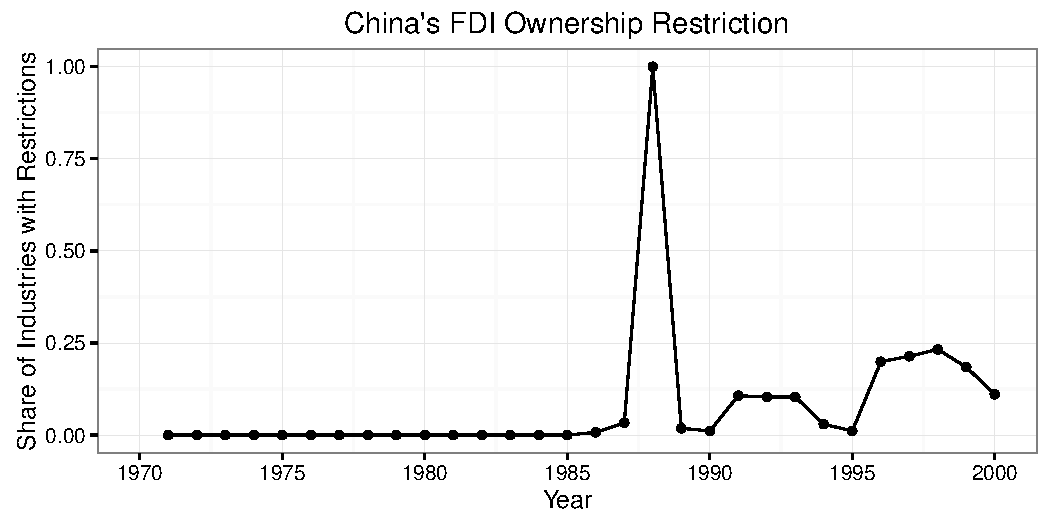
\includegraphics[width=0.75\textwidth,keepaspectratio]{china_fdi_restriction}
\caption{China's FDI Ownership Restriction, as coded in \citet{Pandya2010}.
Prior to 1986, FDI in China was limited to few experimental Special Economic
Zones, and thus not mentioned in US Investment Reports. The sharp spike in 1988
also does not seem to correspond to any actual change in policy, and likely
another artifact of reporting. (See \citet{Zebregs2002} for a historical
overview of China's FDI policy.)}
\label{fig:china_fdi_restriction}
\end{figure}

The two-sided matching model circumvents these thorny measurement issues by
incorporating countries' utility function directly into the model. If we observe
that country $j$ welcomes firms $i_1, i_2, \dots, i_n$ to invest but not others,
we can compare the characteristics of firms $i_1, i_2, \dots i_n$ with the
others to infer country $j$'s preference.


\subsection{Estimating Countries' Preferences for FDI's Technological Intensity}

Laura Alfaro: is all FDI equal? - Use human capital from German firms as a proxy
for all sectors (this works for the OECD sample of that paper, but not more
generally) - Use IPA policy, but this could just be image building by the
country (everyone says that they want advanced manufacturing (cite the picture))

\begin{figure}[!ht] \centering
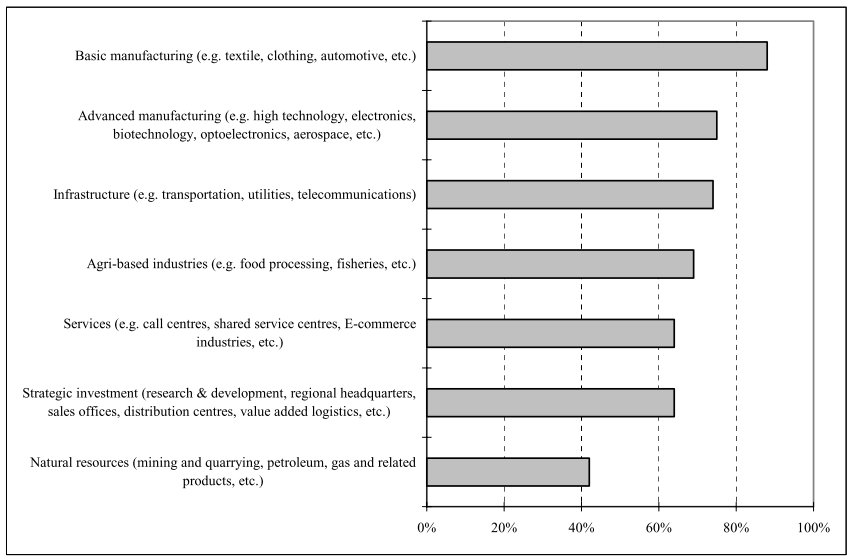
\includegraphics[width=\textwidth,keepaspectratio]{../figure/IPA_target_industries}
  \caption{Target industries by IPA around the world. Because of the image
building aspect of investment promotion, almost all IPAs say that they want to
attract ``advanced manufacturing.'' Therefore, using what is listed as
investment priorities may not be a reliable way to measure countries' preference
for FDI. Source: \citet{UNCTAD2001}}
  \label{fig:IPA_target_industries}
\end{figure}

While the political science literature has focused almost exclusively on the
quantity of FDI, treating all FDI as one homogeneous flow of capital, policy
makers seem to pay much more attention to distinguishing types of FDI.
Commenting on the role of International Investment Agreements (IIAs),
\citet{UNCTAD2015} says, ``Today, increasing the quantity of investment is not
enough. What matters is its quality, i.e. the extent to which investment
delivers concrete sustainable development benefits.'' Governments in developing
countries, from Ghana to China, all offer various forms of tax incentives and
fee waivers to attract FDI that invests in a remote region, brings new
technology, or focuses on exporting \citep{Ricupero2000}. Since 2006, China's
official FDI policy has been ``quality over quantity,'' promoting FDI with
intense R\&D in high-productivity sectors \citep{Guangzhou2011}. Indeed, for
developing countries, the hope is that MNCs will transfer their technologies to
the domestic economy by training workers or partnering with local suppliers.

Despite the importance of disaggregating FDI by its quality, data unavailability
remains the bottleneck. The few existing attempts use detailed data from only
one country or limit the sample to OECD countries \citep{Alfaro2003, Alfaro2007,
Javorcik2004}. With cross-country firm level data now available, we often have
information on the firms' industry or even research and development (R\&D)
expenditure. With the two-sided matching model, I will be able to estimate
countries' preferences for firms' technological intensity. I hypothesize that,
since MNCs' technologies takes time to diffuse to local businesses, a country'
preference of high-tech FDI is shaped by its time horizon.

\section{The literature on Japanese MNCs investment}

Make a graph about the size of Japanese FDI relative to Asia FDI here

Calculate the size of Japanese FDI into several countries (nominator from JETRO,
denominator from IMF)

Relative exchange rate (Takagi2011). Assume that the capital market is
imperfect, that external borrowers face a premium. So if a host country currency
depreciates, inflow FDI will increase because the same amount of source currency
can buy more input in the host country. The relationship is especially strong
between exchange rate and inflow of FDI into industries with a lot of
firm-specific assets. (e.g. Japanese firms buy a US firm with innovation for
cheap, then use that innovation to improve its production back home in yen)

(Originally people don't think exchange rate matter because if you can buy an
asset for cheap in the host country, when you repatriate the profit back to the
home country it's a wash)

FDI is all about the relative factors (because a firm thinks about a country in
terms of how that country is relative to its host). So the two sided matching
framework makes sense

General FDI: Why don't firms export or license, but open their own plant
overseas? Argument is that they have firm-specific asset that cannot be fully
exploited otherwise. A licensee won't be able to exploit the entire asset, both
sides can't agree on a price beforehand (This is the OLI framework,
ownership-location-internalization, also the internationalization hypothesis).
Empirically, firm specific asset is unobservable, so people use R\&D intensity
and advertising intensity instead. R\&D does correlate strongly with
multinationality.


\section{Applying the Two-Sided Matching Model to Japanese MNCs}
\label{sec:application}

In this section, I apply the two-sided matching model to study the investment
location of Japanese firms overseas. The data comes from a dataset compiled by
Andrew Delios from \textit{Kaigai Shinshutsu Kigyou Souran} (Japanese Overseas
Investments-by Country), between 1986-1999 editions, a publication that contains
information about the foreign affiliates of listed Japanese firms.\footnote{I
thank Professor Andrew Delios for generously sharing the data.} Tokyo Keizai,
Inc. collect these data via annual surveys of the overseas operations of both
listed and non-listed firms. This database is reputed to include all Japanese
firms overseas \citep{Yamawaki1991}. \citep{Delios2001} compares the coverage of
the Japanese Overseas Investment with other sources of publicly listed firms and
found that 98.5\% of public firms are included, which has 99.5\% of the foreign
subsidiaries. Since there is no public information on non-public firms, they
cannot check the coverage of the Japanese Overseas Investment for these firms.
However, the result for the public firms makes us confident that our data is
close to the population of Japanese FDI overseas. This dataset has been used to
study X, Y, and Z \citep{Delios2000}. \footnote{There are similar datasets if
scholars want to replicate this study in other context. On a global scale, the
ORBIS dataset claims to have data of FDI firms across countries. (cite the paper
that I reviewed). However, there are concerns about its data quality, given that
the data is collected via public governmental or municipal sources. Due to the
differences of reporting across jurisdiction, the data quality is much less
consistent than the Japanese Overseas Survey. For the US, there is a census of
US firms overseas, which should be similarly high quality. However, this dataset
requires citizenship. Tokyo Keizai, Inc. also continue to publish this data
series. However, the cost is prohibitive and require understanding Japanese to
work with.}



Sample choices:

- I only use the data of subsidiaries that are founded in year 1996 (which is
different from the list of companies who are in existence in year 1996).
Reasons: + the utility function is only modeled as a linear combinations of the
country / firms covariates. It does not take into account the cost of uprooting
a firm to move to another country once they are already there. This is important
for FDI because, unlike equity investor, FDI are less foot-loose. Indeed, the
fact that it is not footloose is an important quality of FDI that's appealing to
countries (cite). The political economy literature on FDI has also derived its
insights largely from this ``obsolescing bargain'' problem, so it's important
that our model takes this into account. In past applications of the two sided
matching approach, researchers use a random sample in time (i.e. a sample of all
couples who's married in a certain year), which is fine, because the cost of
leaving a job or leaving a partner may not be too onerous. However, for FDI,
this fixed cost is more central. By limiting the sample to the firms who are
founded in 1996, we examine their decisions as they are all looking for
potential locations.\footnote{Of course, a subsidiary's foundation year in 1996
does not preclude the decision process to happen outside of this year. However,
I consider this a reasonable approximation, given that many country
characteristics, especially the political and institutional ones, do not change
drastically within a window of several years.}

+ the data is largest for this year. (some summary statistics here). There may
be some concerns about this year being a special year, in the year leading up to
the 1997 Asian Financial Crisis. But 1) we're only looking at manufacturing
firms, not equity investors or land developers, 2) FDI during the crisis is
largely the same as before the crisis \citep{UNCTAD1998}. Indeed, this is
because FDI firms are largely looking at countries' fundamentals, such as labor
cost, market potential, and thus not affected by the fluctuations in the
financial markets. Essentially, the types of firms that invest before, during,
and after crisis are still the same types of firms.\footnote{One potential
concern is that our data does not capture the firms who thought about making an
investment but decided not to. This could be a problem if the MNCs in our
dataset is the most risk-seeking firms, then essentially we've only estimated
the preference of the very risk-seeking or the very risk-averse firms. AFC too
high short term interest, too high local currency that is fixed. However, the
exit rate of Japanese firms in Thailand, the epicenter of the financial crisis,
is the same, indicating that the types of firms who invest are not so affected
by the financial crisis. Looking at the exit is the reverse way of looking at
who would have invested but didn't. \citep{Delios2001}}

+ I only consider Japanese FDI into East Asian and Southeast Asian economies to
make sure that it's realistic to say that all these companies have the same
preference parameters. \citep{Pak2005} finds that Japanese FDI in the West seeks
to augment their global competitiveness, while Japanese FDI in the East focuses
on exploiting their core competencies. Japanese FDI in the West are ones with
oligopolistic power in their domestic market (so they are in a strong position
to compete) and require R\&D and marketing capabilities. They have different
level of equities. This suggests that the two types of firms are fundamentally
different.\footnote{Even though the difference in theory could be due to the
preference of the countries. However, it doesn't make sense why the level of
Japanese ownership is also different (because countries would not care about
this).}

The final sample includes 6474 Japanese foreign affiliates in 2003, spreading
across 37 countries, with China and the US leading as the two top destinations
for Japanese MNCs (Table \ref{tab:list_of_countries}).

For firms' characteristics that countries consider, I include:

\begin{itemize}
\item Capital size (in US\$): A main argument for the benefit of FDI is that it
brings capital to the country, improving labor productivity. MNCs' capital is
especially important for developing countries, which cannot muster much domestic
capital from their poor population. The capital size of a firm is included in
the Japanese Overseas Business dataset.

\item Labor size: Similarly, a reputed benefit of FDI is that it creates jobs,
generating not just economic growth but also increasing the government's
popularity among the populace. The total number of employees of a firm is
included in the Japanese Overseas Business dataset.

\item Technology intensity: I proxy for a firm's technology intensity by the
industry to which it belongs. \citet{OECD2009} categorizes ISIC industries into
four levels of technology intensity---low, medium low, medium high, and
high---according to the level of R\&D expenditure divided by sales. I convert
the industry classification of firms in my data from SIC 3 to ISIC and
categorize their technology intensity from 1 to 4, with 1 being low and 4 being
high. On several occasions, one industry in SIC 3 matches to multiple ISIC (rev
3) industries or none at all. In the former case, I take the average across
matched ISIC industries. In the latter case, the data is missing and later
removed from the analysis.\footnote{\cite{Bergstrand2007} discusses the
difference between R\&D intensity and advertising intensity, and find that R\&D
intensity is higher for manufacturing firms compared with consumer product
firms. Plus R\&D intensity is much more important for firms' performance than
advertising intensity.}\footnote{Definition of R\&D intensity: the amount spent
on R\&D as a percentage of sale}

\item Export intensity (ratio of export to sale):
\end{itemize}

Summary statistics table for these covariates.


For countries' characteristics that firms consider, I include:

\begin{itemize}
\item Market size: MNCs are expected to prefer countries with a large market
size, which present MNCs with many potential customers. Indeed, this has been
often cited as the allure of China to MNCs \citep{Luo2010}, as well as confirmed
in larger studies. This is also a major variable in the gravity model, which has
become a standard model for analyzing FDI flows. \citet{Bergstrand2007} provides
the theoretical framework for the use of gravity model. I follow the standards
in the literature and include log GDP (constant 2005 US\$), taken from the Penn
World Table.\footnote{An advantage of the Penn World Table is that it compiles
data for Taiwan, an important destination that the World Bank Development
Indicators does not include.}

\item Level of development: MNCs are expected to prefer countries with a high
level of development. A developed economy has consumers with high purchasing
power and better infrastructure. It can also measure capital abundance, in which
case a higher GDP per capita imply less flow because the simple model of FDI
frames FDI as the movement of capital from the capital rich countries to the
capital poor countries. To measure development, I use log GDP per capita
(constant 2005 US\$) from World Development Indicators.

\item GDP growth may be a proxy of potential returns,

\item Labor quality: As one primary factor of production, labor matters greatly
to firms' productivity and profit. To measure labor quality, I use the average
years of schooling of adult, taken from the UNDP's Human Development
Report.\footnote{Since Taiwan is not included in UNDP's and World Bank's data, I
collected its statistics from the Taiwanese Statistical Website.}

\item Democracy: Democracy has been a mainstay in the political science
literature on FDI. Scholars have argued that MNCs want to invest in democratic
regimes for various reasons, including stable policy, credible commitment, and
strong property rights \citep{Ahlquist2006, Li2003, Jensen2003}. On the other
hand, recent works have also argued that democratic regimes want FDI more than
autocratic regimes \citep{Pandya2016}. Thus, it is unclear whether the observed
high level of FDI in democracies is due to the push or the pull factors. By
controlling for countries' preference in the two-sided matching model, I can
better estimate the effect of democracies on firms' utility. I measure democracy
using the binary Demoracy \& Dictatorship, developed by \citet{Cheibub2009b}.
\end{itemize}

\section{Result}
\label{sec:result}

\begin{figure}[!ht] \centering
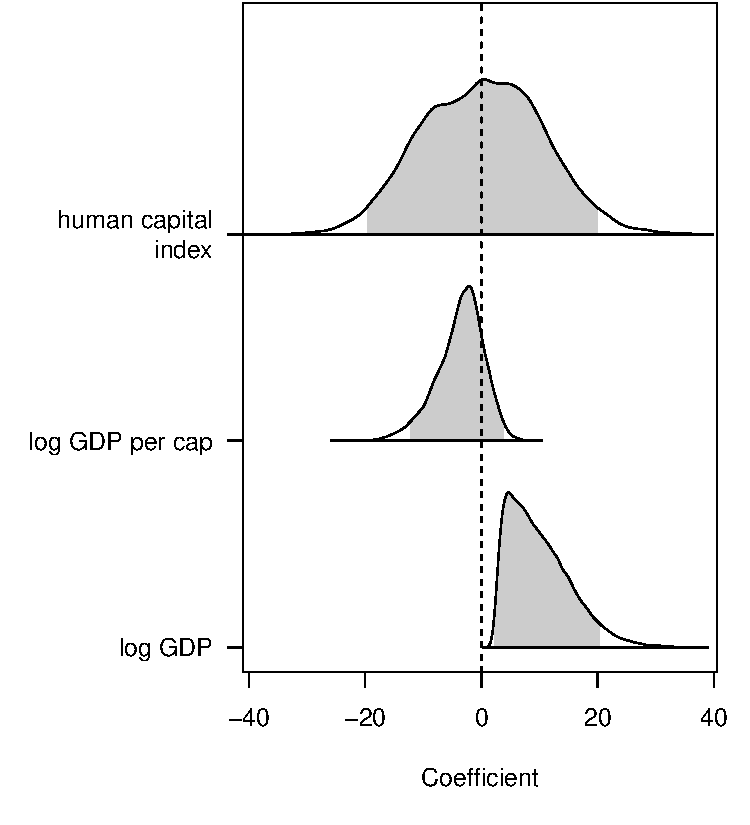
\includegraphics[width=0.75\textwidth,keepaspectratio]{japan96_alpha}
  \caption{Preference of MNCs for countries' characteristics. The density plot
and the shaded region show the posterior distribution and the 95\% credible
interval.}
  \label{fig:japan96_alpha}
\end{figure}

\begin{figure}[!ht] \centering
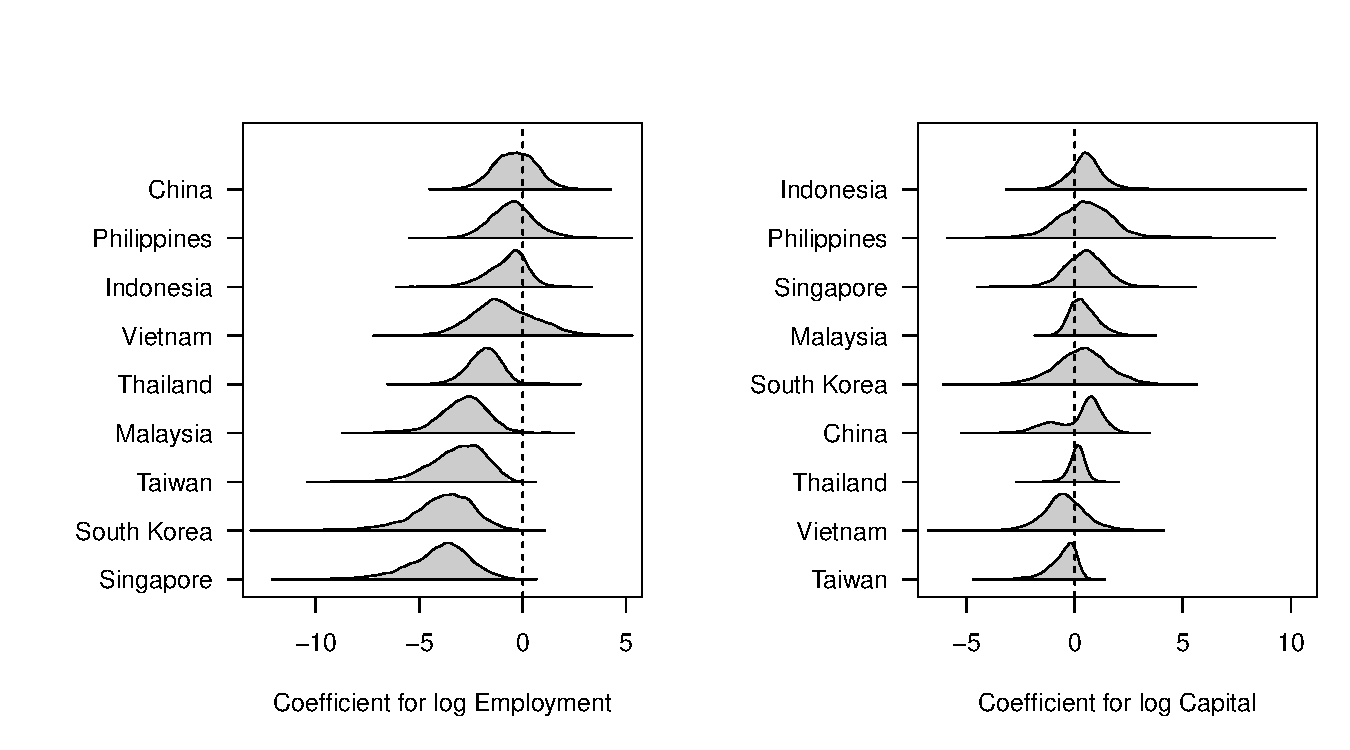
\includegraphics[width=\textwidth,keepaspectratio]{japan96_beta_ltemp_luscptl}
  \caption{Preference of countries for firms' size, measured by their labor
force (left) and capital (right). The density plot and the shaded region show
the posterior distribution and the 95\% credible interval.}
  \label{fig:japan96_beta_ltemp_luscptl}
\end{figure}

\begin{figure}[!ht] \centering
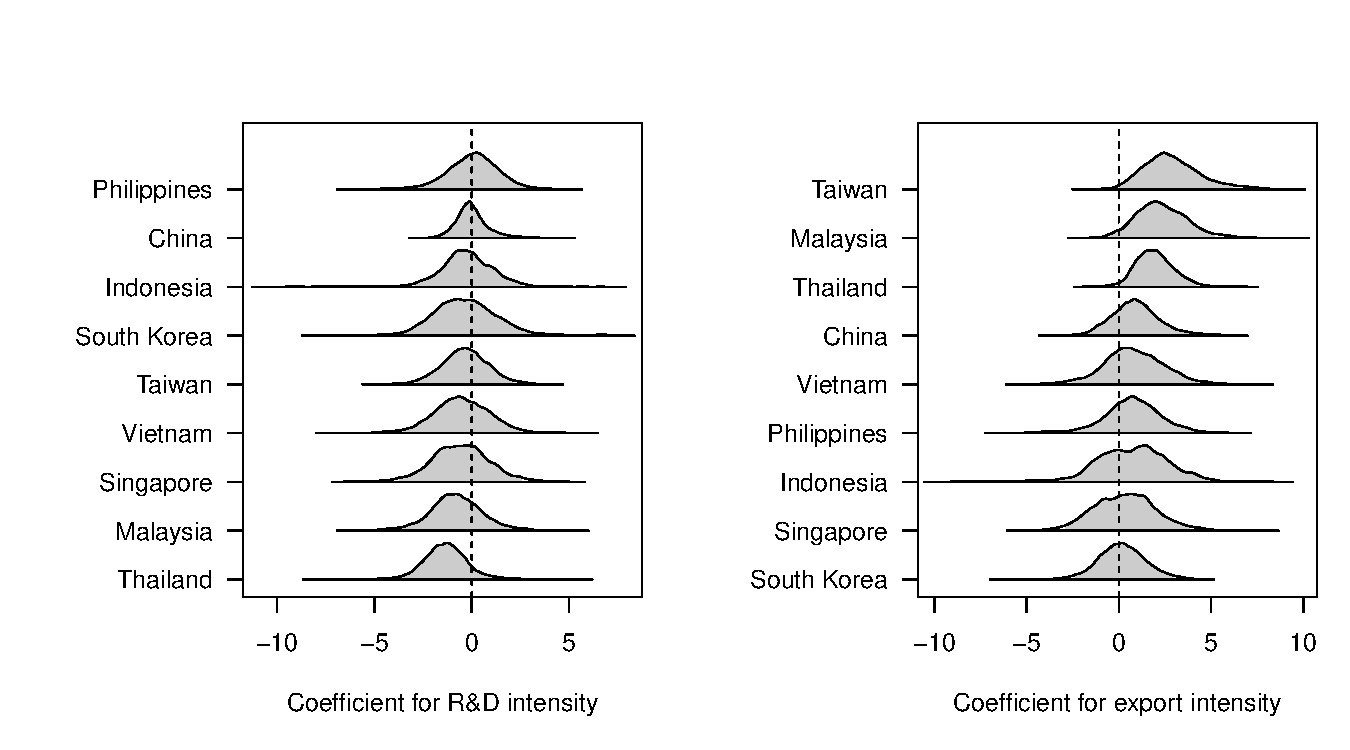
\includegraphics[width=\textwidth,keepaspectratio]{japan96_beta_intrd_intexp}
  \caption{Preference of countries for firms' intangible assets, i.e R\&D
intensity (left) and export intensity (right). The density plot and the shaded
region show the posterior distribution and the 95\% credible interval.}
  \label{fig:japan96_beta_intrd_intexp}
\end{figure}

\begin{figure}[!ht]
  \centering
  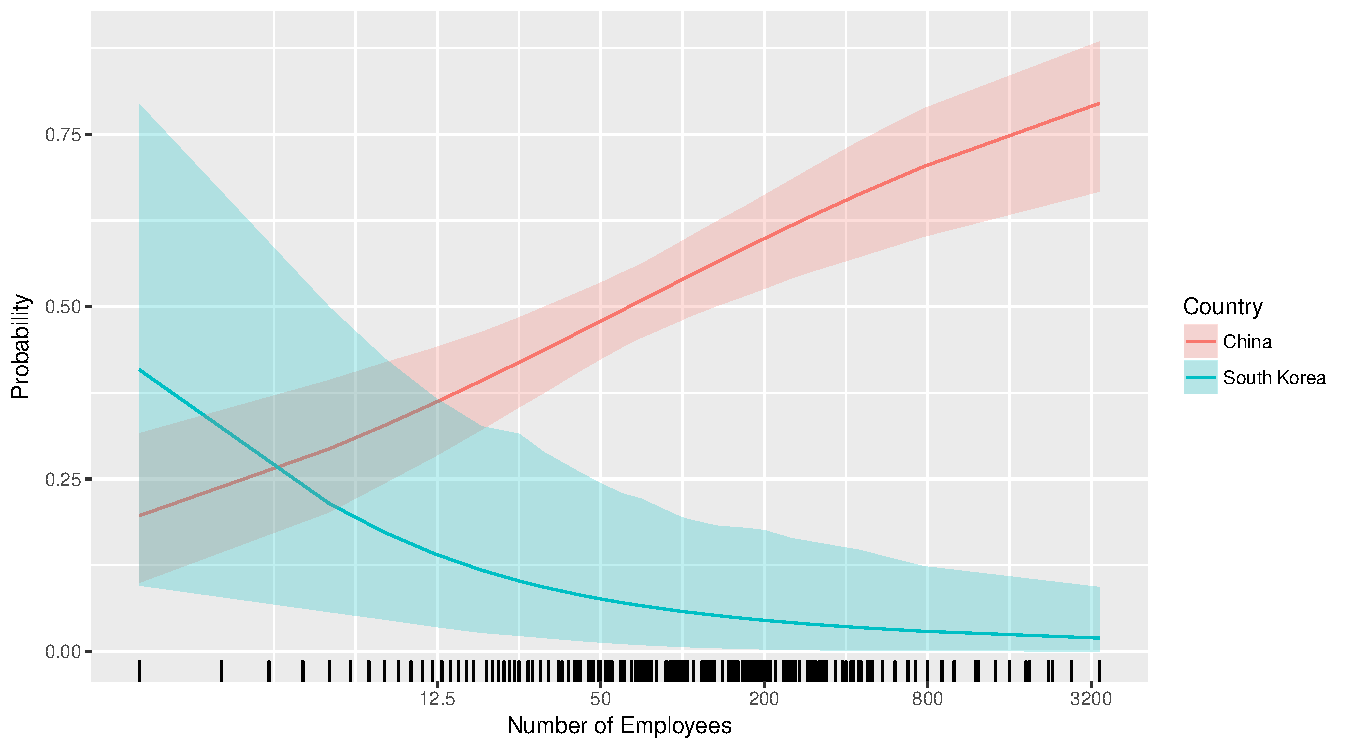
\includegraphics[width=\textwidth,keepaspectratio]{../figure/japan96_effect_of_temp}
  \caption{The effect of employee size on the probability to be offered by China
    and South Korea}
  \label{fig:japan96_effect_of_temp}
\end{figure}

\section{Model fit}
\label{sec:model_fit}

\begin{figure}[!ht] \centering
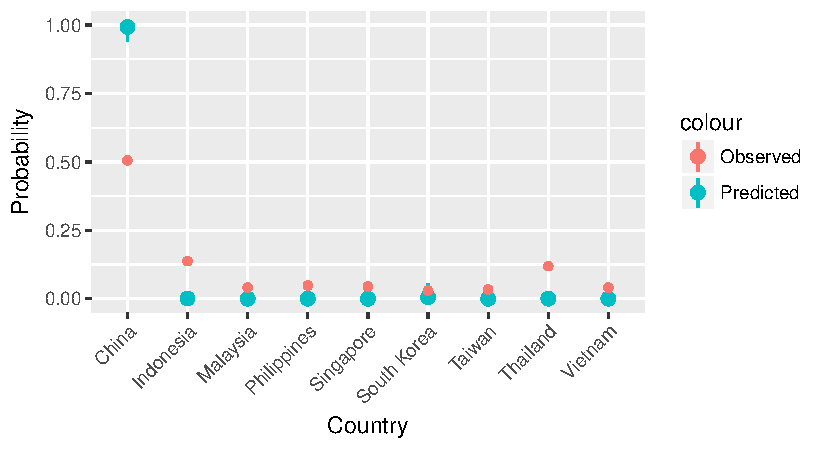
\includegraphics[width=\textwidth,keepaspectratio]{japan96_prob_being_chosen_by_MNC_one_sided}
  \caption{Predicted and observed probabilities that an MNC chooses to locate in
a country, unconditional on the preference of countries. The point and the error
bar show the posterior mean and the 95\% credible interval.}
  \label{fig:japan96_prob_being_chosen_by_MNC_one_sided}
\end{figure}


\begin{figure}[!ht] \centering
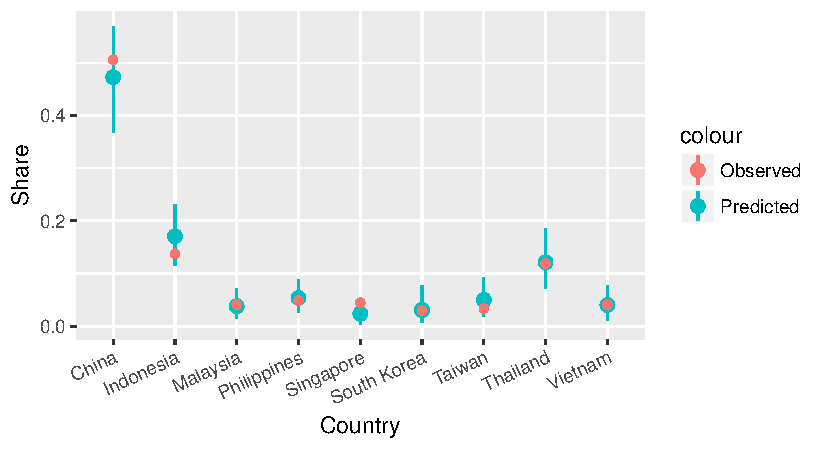
\includegraphics[width=\textwidth,keepaspectratio]{japan96_prob_being_chosen_by_MNC_two_sided}
  \caption{Predicted and observed probabilities that an MNC chooses to locate in
a country, conditional on the preference of countries. The point and the error
bar show the posterior mean and the 95\% credible interval.}
  \label{fig:japan96_prob_being_chosen_by_MNC_two_sided}
\end{figure}

Profiles of firms

\begin{figure}[!ht] \centering
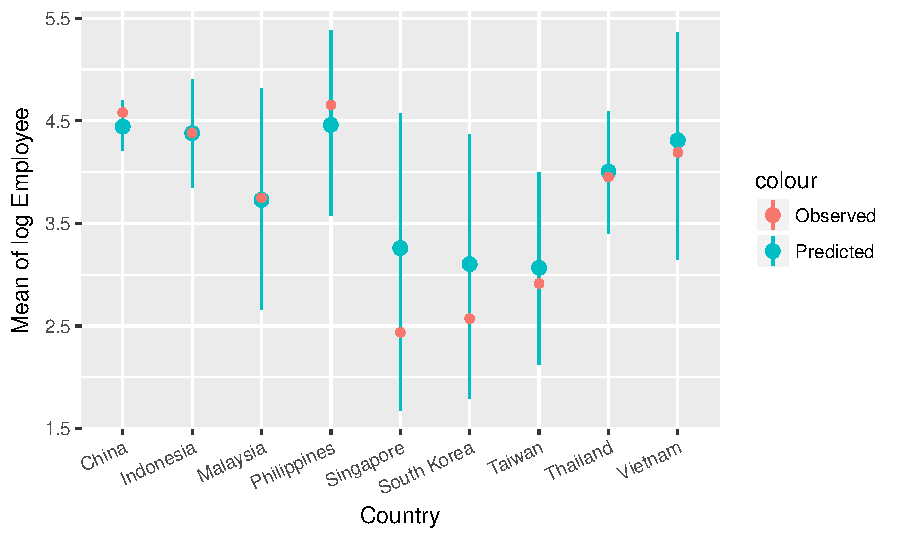
\includegraphics[width=\textwidth,keepaspectratio]{japan96_sim_mean_ltemp}
  \caption{Average of MNCs' labor size across countries. The point and the error
bar show the posterior mean and the 95\% credible interval.}
  \label{fig:japan96_sim_mean_ltemp}
\end{figure}

\begin{figure}[!ht] \centering
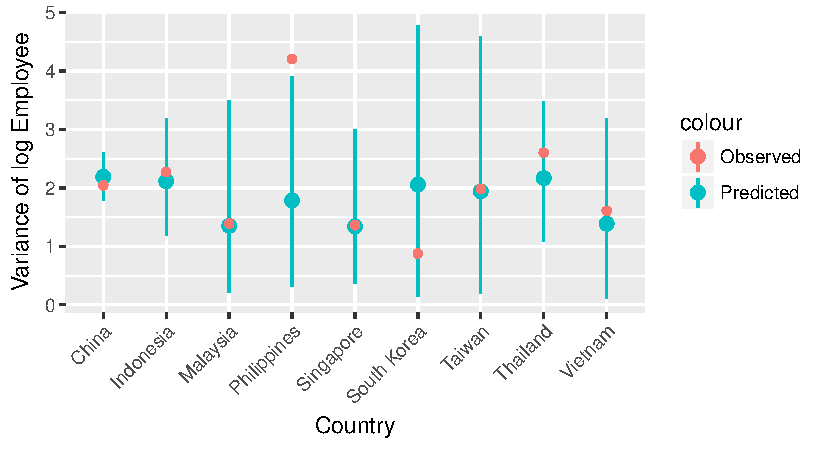
\includegraphics[width=\textwidth,keepaspectratio]{japan96_sim_var_ltemp}
  \caption{Variance of MNCs' labor size across countries. The point and the
error bar show the posterior mean and the 95\% credible interval.}
  \label{fig:japan96_sim_var_ltemp}
\end{figure}

\section{Political determinants of FDI}

\citep{Nunnenkamp2002} finds that for developing countries market based factors
are still the most important

\section{Conclusion}
\label{sec:conclusion}

In this paper, I propose the two-sided matching model to estimate firms' and
countries' preferences, solving three persistent issues in the literature of
FDI's political determinants. The results indicate that, for Japanese MNCs, only
a country's level of development matters and not its market size, labor quality,
or regime type. This finding suggests that we should take a closer look at the
relationship between democracies and MNCs. Since previous works in the
literature have not controlled for countries' preferences, they may have
mistaken democracies' love for FDI as FDI's fondness for democracies.

On the other hand, the model's estimation of countries' preference remains
lacking. Since each country has its own set of parameters, the parameter space
seems too large for the current implementation of the Metropolis-Hastings
algorithm to fully explore. Several solutions are possible. First, we can
collapse countries into categories of interest, e.g. regime types, (categorical)
time horizon length. Second, we can build a hierarchical model, modeling
countries' preferences as draws from a common distribution. Such model will
allow us to pool information across countries and reduce the parameter space.

%%% Local Variables:
%%% mode: latex
%%% TeX-master: "../AnhLe_dissertation.tex"
%%% End: